\documentclass[a4]{article}
\usepackage[top=2cm,right=4cm,bottom=2.5cm,left=2cm]{geometry}\setlength{\parindent}{0cm}
\usepackage[utf8]{inputenc}
\usepackage{cite}
\usepackage{amsmath,amssymb,amsfonts}
\usepackage{algorithmicx}\usepackage{algpseudocode}
\usepackage{graphicx}
\usepackage{textcomp}
\usepackage{xcolor}
\usepackage{ulem}
\usepackage{enumitem}
\usepackage{fancyvrb}
\usepackage{caption}
\usepackage{subcaption}
\usepackage{url}
\usepackage[hidelinks,breaklinks]{hyperref}
\usepackage{booktabs}
\usepackage{multirow}
\usepackage{lscape}

\newcommand{\vthierry}[2]{{\color{magenta} #1} \sout{#2}}
\newcommand{\fred}[1]{{\color{green} #1}}
\newcommand{\chloe}[1]{{\color{blue} #1}}
\newcommand{\axel}[1]{{\color{brown} #1}}
\newcommand{\deq}{\stackrel {\rm def}{=}}
\newcommand{\tab}{\hphantom{~}}
\newcommand{\drawn}{\stackrel {\text{drawn}}{=}}
\newcommand{\eqline}[1]{~\vspace{0.1cm}\\\centerline{$#1$}\vspace{0.1cm}\\}
\newcommand{\hhref}[1]{\href{#1}{#1}}

\title{Where is Aristotle in our brain ? On biologically plausible reasoning embedded in neuronal computation.
\thanks{Supported by Inria, AEx AIDE \url{https://team.inria.fr/mnemosyne/en/aide}.}}
\author{Chloé Mercier$^1$\and
%\inst{1}\orcidID{0000-0002-5069-3138}  \and
% # Et selon l'orientation du papier …
%Gabriel Doriath Döhler$^1$\and
%\inst{1}\orcidID{0000-0000-0000-0000}
%Hugo Chateau-Laurent$^1$\and
%\inst{1}\orcidID{0000-0002-2891-0503}
%Frédéric Alexandre$^1$\and
%\inst{1}\orcidID{0000-0002-6113-1878} \and
Thierry Viéville$^1$\\
%\inst{1,2}\orcidID{0000-0003-1031-3572}
\\%\affiliations
$^1$Mnemosyne Team, Inria Bordeaux, U. Bordeaux, LaBRI and IMN \\
\\%\emails
firstname.lastname@inria.fr
}
\date{Before end 2022 :)}

\begin{document}

\iftrue

\maketitle

\begin{abstract}

Human cognition involves tightly interleaved numerical but also logical computations. How can the brain implement such processing is an important issue, and we would like to address some aspect here, combining two approaches.

On one hand, ontology related languages allow us to describe symbolic structured knowledge and perform logical inference using entailment rules. To what extent this could provide a rather natural representation of some aspect of usual human reasoning is an open question, that we are going to discuss here, considering a modal logic generalization.

On the other hand, spiking neural networks are biologically plausible implementations of brain circuits computations, that can be interpreted as a symbolic architecture providing a way to manipulate symbols embedded as numeric vectors that carry semantic information. In the present work, we consider such Vector Symbolic Architecture (VSA) allowing us to describe neural implementation at an algebraic level, in order to show that modal logic reasoning can naturally emerge from usual distributed calculus, yielding to neurosymbolic computations.

This development illustrates that modal logic reasoning can come with usual neural computation, by being embedded in brain computational processing, enriching brain neurosymbolic deduction, especially in problem solving.

\end{abstract}

{{\bf Keywords:} Ontology, Modal Logic, Semantic Pointer Architecture, Abstract thought, Neurosymbolism, Problem-solving.}

\section{Introduction}

\subsection{Describing cognitive knowledge and inference}

\paragraph{From sensori-motor processing to logical reasoning.}

It is well-known as reviewed, e.g., in \cite{ness_knowledge_2007}, that, roughly speaking, human logical reasoning emerges progressively from sensorimotor association, with the formation of stable concepts, even at a symbolic level, before being able to manipulate them at a concrete level, performing inductive reasoning, up to more formal deductive reasoning. Furthermore, as pointed out in \cite{arnett_adolescence_2001}, there is a cultural bias, since not all persons in all cultures feel the need to develop formal logical operation competences as it, and obviously most people do not use such formal operations in all aspects of their lives. However, as discussed in, e.g., \cite{keefer_metaphor_2016}, deductive reasoning, especially for goal-driven behavior, is deeply interlaced with heuristic deduction, involving analogy and metaphor. Furthermore, as deeply studied by, e.g., \cite{purves_interplay_2001}, the experience of conscious or subconscious emotion has a powerful influence on rational decisions, including the choice of alternatives in deductive reasoning. Does this means that the human brain does {\em not} need to develop deductive reasoning, except for singular cultural need (e.g., for scholarship constraints or to practice formal science)? Our understanding is that the situation is not binary. We definitely need to make deductions to solve every day life problems, while the elements we briefly reviewed here, demonstrate that such deduction are not Boolean (either true or false) but related to a given context, weighted by a certain level of belief, and biased by motivational elements, in the wide sense.

We are going, in this study, to attempt to reconcile deductive reasoning with such cognitive mechanism of inference, up to a biologically plausible neuronal implementation.

\paragraph{Modal logic and belief representation.}

\paragraph{Knowledge representation}

From early artificial intelligence knowledge representation as, say, frames avowed previously, to modern web semantic data structures, the basic idea of symbolic representation is to consider symbols representing objects and express the knowledge by relations, i.e., triple statements of the form {\tt \$subject \$predicate \$object.}, as schematized in Fig.~\ref{triple}.

\begin{figure}[htbp]
\centerline{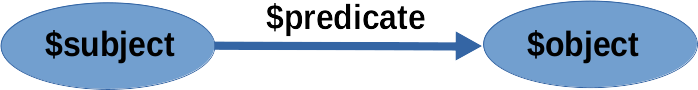
\includegraphics[width=0.5\textwidth]{figures/triple.png}}
\caption{Atomic representation of knowledge: To express a bean of knowledge regarding a symbol, the subject, we define a quality, with a predicate, with an object as attribute (i.e., a data value or another symbol).}
\label{triple}
\end{figure}

Following, e.g., \cite{gardenfors_conceptual_2004}, we start with the simple common idea that a concept can be defined by ”quality dimensions”, i.e., attributes with some typed value. The object can be either a qualitative or quantitative ``data'', or another object, stating relations between objects. This is also the basic syntax of ontology languages. In the brain, such quality dimensions are usually anchored in sensori-motor feature spaces \cite{freksa_strong_2015}, in coherence with the present presentation. Furthermore, given a concept, as developed in \cite{gardenfors_conceptual_2004}, this choice of representation induces the notion of prototypes, that allows to represent the state space region corresponding to the concept.

Predicates can be generic, in the sense of e.g. \cite{mcclelland_parallel_2003}, defining hierarchical taxonomy using the “{\tt is-a}- predicate, as in almost any such language, but also capability “{\tt can}”, extrinsic qualities “{\tt has}” and intrinsic qualities “{\tt is}”, thus four general predicates. They also can be unconstrained, as in the RDFS framework (see .e.g. \cite{noy_ontology_2001} for an introduction), describing any property and in that case properties also form a taxonomy\footnote{For instance stating that {\tt Amid is-a-descendant-of Yang-Li} implied that {\tt Amid is-the-family-of Yang-Li} the former property being a sub-property of the latter. This examples also illustrates that such properties have meta-property, such as being transitive or symmetric.}. On the reverse, as a limit case, we can consider only the fact that subject and object are in relation without considering the predicate and the direction of the relation.

An important point is that qualities can be hierarchical because the value has itself some qualities, for instance a quantitative physical value is not only a ``number'' stating the current or default value, whereas the unit is to be made explicit and the value precision also, when not its bounds. In terms of data structure this forms a tree, and the whole data structure is a set of tree, i.e. a forest, thus a graph.

We are going to specify how we can represent such symbolic information at a biologically plausible level in the present study, thanks to vector symbolic architectures introduced now.

\subsection{Representing neuronal activity at a symbolic level}

As a possible entry to consider a biologically implementation at a symbolic level,  Vector Symbolic Architectures (VSA) were introduced as a way to manipulate symbolic information represented as numeric vectors (see e.g. \cite{levy_vector_2008} for an introduction). VSAs have been proven helpful to model high-level cognition and account for multiple biological features \cite{gayler_vector_2003,eliasmith_how_2013}. More specifically, the Semantic Pointer Architecture \cite{eliasmith_how_2013} instantiates so-called semantic pointers (i.e. vectors that carry semantic information) and their manipulation in networks of spiking neurons. This approach makes a significant step towards the unification of symbolic and sub-symbolic processing in that it provides a way to translate the former into the latter. Consequently, complex knowledge representation in the form of compositional structures that are traditionally restricted to symbolic approaches can now be distilled in numerical and even neural systems \cite{crawford_biologically_2016}.

\paragraph{The basic idea of distributed representation.} 

How can we represent a symbol in a neuronal assembly ? A localistic representation (one neuron or neuron group by symbol) is not realistic, and the basic idea is that a symbol corresponds to a pattern of activity of the whole assembly. Let us consider a spiking neuron network and quantify its activity by some statistics, e.g. the neuron rates, or higher order statistics (see e.g. \cite{cessac_dynamics_2008} for a discussion). As developed in \cite{eliasmith_neural_2002}, this includes timing codes and population codes (i.e., relative timing codes between neurons) and the authors show how with their developed Neural Engineering Framework (NEF) we can collect this high dimensional set of bounded quantitative values, which can be normalized, as unit stochastic vector in a huge dimensional space (of a few thousands for a biological neural map, often a few hundred at the simulation level), defining a Semantic Pointer Architectures. This includes temporal representation in spiking neurons systems, not only a rate representation. The key point is that comparing to other representation, e.g., based on synchrony within the neural assembly, the NEF alternative is much more scalable.

In the present study, we consider these developments as prerequisites and will simply consider that neural assembly activity is represented by a high dimensional unary stochastic vector. We also need to specify transformations and will define them at this abstract algebraic level. Mainly, following \cite{mercier_ontology_2021} we will consider auto-association mechanism, as developed in \cite{stewart_biologically_2011} and functional transformations as detailed in \cite{eliasmith_neural_2002}, their development being based, in a nutshell, on parameterized kernel based approaches.

\paragraph{On numerical versus semantic grounding.} 

A step further, how it is that, in the brain, symbols considered here get their meanings? We will not address this issue here, but would like to clarify some points. First of all, in neurosymbolic studies as reviewed in \cite{garcez_neurosymbolic_2020} grounding is understood as the process to embed symbolic computations onto real-valued features \cite{badreddine_logic_2021}, because it allows to provide a semantic interpretation or model (in the sense of a model of set of logical assertions) of the symbolic system. This means that it is no more an abstract set of assessments (potentially without any concrete implementation) but something that correspond to a real formal object.

This differs from the symbol grounding problem as reviewed and discussed in \cite{taddeo_solving_2005}, where symbols are linked to their meaning, which involves the capacity to pick referents of concepts and a notion of consciousness. In a nutshell, this is still an open problem, that we are not going to solve here. However, proposals to link abstract symbolic to the neuronal reality, enrich the issue about how mental states can be meaningful. Furthermore, the fact our abstract representation is anchored in sensory-motor features, is also a link between symbols and their potential referent. A step further, when we represent concepts, the chosen design choice associates prototypes, allowing to anchor an abstract element to a concrete example.

Another aspects not targeted by the present study, is the emergence of symbols, i.e., the fact that a symbolic representation emerges from a biological or any physical system in interaction with its environment. The issue is addressed in \cite{rougier_implicit_2009} for a toy experiment, emphasizing that to address such issue, we must avoid to explicitly embed any symbol anywhere in the model, a priori or a posteriori. Here, we do not address the emergence issue, but in a sense a {\em feasibility} issue: to what extents event sophisticated symbolic processing can be anchored in numerical processing, not only rudimentary operators. We also address an {\em interpretation} issue, i.e. to what extends sub-symbolic sensory-motor anchored processing corresponds to symbolic processing, as discussed in the sequel.

Our approach thus does not solve the grounding problem, but in some sense what we can called the ``anchoring'' problem of relating symbols with the neural substrate which activity allows their grounding.

\fi

\section{Methods}

Let us first discussed how we encode symbols, basic knowledge and their degree of belief and then define transformation on these symbols. The key idea is to study to what extent symbolic reasoning on symbols may correspond to algebraic operations implemented via numerical computation, based on a framework introduced in \cite{eliasmith_how_2013}.

\subsection{Symbolic information encoding}

\paragraph{Symbol encoding.}

At the numerical level, each symbol is implemented as a randomly drawn fixed unit $d$-dimensional vector, $\mathbf{x} \in {\mathcal R}^d$. Typically $d\simeq 100 \cdots 1000$ and we expect to manipulate $k\simeq 100 \cdots 10000$ symbols, at the simulation level. In a cortical or brain map, the order of magnitude is higher since the vector corresponds to the neural map activity (thus closer to $10^{5\cdots 6}$ and the number of encoded symbols depends on which map is considered. 

The vector components are drawn from a normal distribution, divided by $\sqrt{d}$, in order to have a $O(1)$ magnitude.

A similarity measure is now introduced in order to semantically compare two vectors. Classically, the cosine similarity (i.e., normalized dot product, denoted $\cdot$) is used to compute the semantic similarity between two unit vectors:
\eqline{\mathbf{x} \cdot \mathbf{y} \deq \mathbf{x}^\top \mathbf{y}}
where $\mathbf{x}^\top$ denotes the transpose of $\mathbf{x}$. This will be sufficient here.

The key property is that, provided that the space dimension $d$ is large enough, two randomly chosen different vectors will be approximately orthogonal. More precisely,
\eqline{{\bf x} \cdot {\bf y} \sim {\mathcal N}(0, O(1/d)),}
i.e., follows a centered normal distribution  \cite{schlegel_comparison_2020}, while by construction ${\bf x} \cdot {\bf x} \simeq 1$.

This allows us to define a hypothesis to decide whether the ${\cal H}_0$ hypothesis ${\bf x} \cdot {\bf y} = 0$ can be rejected, we are in the situation of a two-tailed ``z-test'', with the alternative hypothesis ${\cal H}_0$ that ${\bf x} \cdot {\bf y} \neq 0$. Here the z-score\footnote{Given a distribution the z-score for $d$ samples is defined as 
\eqline{z \deq \frac{\bar{X} - \mu}{\sigma / \sqrt{d}}}
with here the expected means is $\mu = 0$ the a priori standard-deviation is $\sigma = O(1/d)$ and the experimental mean $\bar{X} = ({\bf x} \cdot {\bf y})$ value is obtained from the dot-product.} is obviously, with $d$ samples and a known standard deviation of order of magnitude $O(1/d)$:
\eqline{z \equiv \sqrt{d} \, ({\bf x} \cdot {\bf y}),}
follows an almost distribution as it can be easily verified numerically, in Fig.~\ref{z_score}, left column. A step further considering two vectors which are not independent, but have an angular dependency we can numerically verify, in Fig.~\ref{z_score}, right column.

\begin{figure}[htbp]
\centerline{\begin{tabular}{cc}
 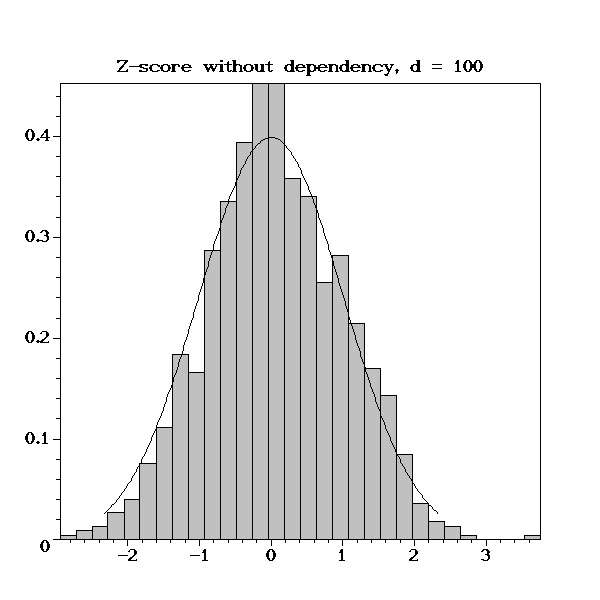
\includegraphics[width=0.5\textwidth]{figures/z_score_2.jpg} &
 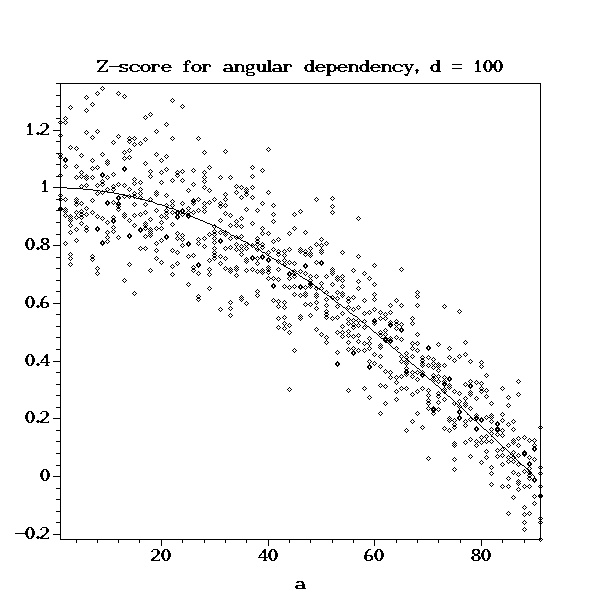
\includegraphics[width=0.5\textwidth]{figures/z_score_2a.jpg} \\
 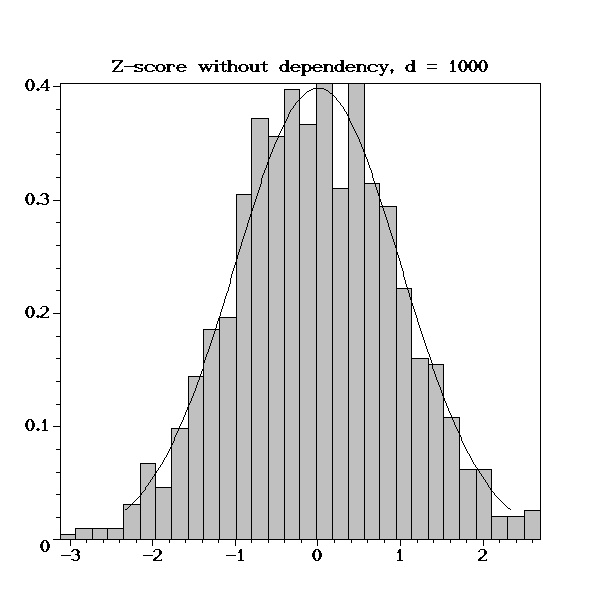
\includegraphics[width=0.5\textwidth]{figures/z_score_3.jpg} &
 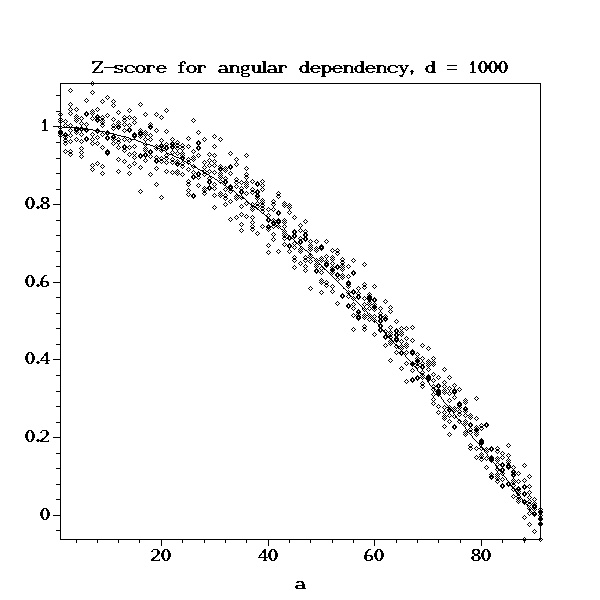
\includegraphics[width=0.5\textwidth]{figures/z_score_3a.jpg} \\
\end{tabular}}
\caption{Numerical observation the dot product of two random vectors for $d=100$ in upper row and $d=1000$ in the lower raw. Left columns show the histogram of the z-score $\sqrt{d} \, ({\bf z} \cdot {\bf y})$ for two normal vectors, in comparison with a normal distribution, these experimental distributions have a kurtosis about 10\% lower that 3, as expected for a normal distribution. Right columns show the $({\bf z} \cdot {\bf y})$ for a vector ${\bf z} \deq \cos(\theta) \, {\bf x} + \sin(\theta) \, {\bf y}$, given two random vectors ${\bf x}$ and ${\bf y}$ as a function of the angular dependency $\theta$, compared to $\cos(\theta)$ drawn as a thick curve.}
\label{z_score}
\end{figure}

This allows on one hand to consider, for instance, a $\pm 2$ threshold on the z-score to have a confidence interval better than $99\%$, and to relate the similarity estimation to an angular dependence between two vectors, as detailed in Fig.~\ref{z_score}.

\paragraph{Modality encoding.}

Based on this, most VSA approaches consider that 2 vectors \textbf{x} and \textbf{y} are semantically equivalent when this similarity $\tau$ equals to 1, but with ways to interpret the result. Here we enrich the notion of being either false or true, by a numeric representation of, e.g., partial knowledge, as illustrated in Fig~\ref{possibility-necessity}. The true value corresponds to 1 (fully possible and fully necessary), the false value to -1 (neither possible nor necessary, i.e., impossible) and the unknown value to 0, which corresponds to a fully possible but absolutely not necessary value. This representation has been designed to be compatible with the ternary Kleene logic, beside being also coherent with respect to the possibility theory, as discussed in detail in appendix~\ref{possibility-representation}, where this deterministic representation of partial knowledge is generalized in order to also include a probabilistic representation (using a 2D representation). In particular, we show that our representation is in one to one correspondence with the dual notion of necessity and possibility of the standard theory.

\begin{figure}[htbp]
\centerline{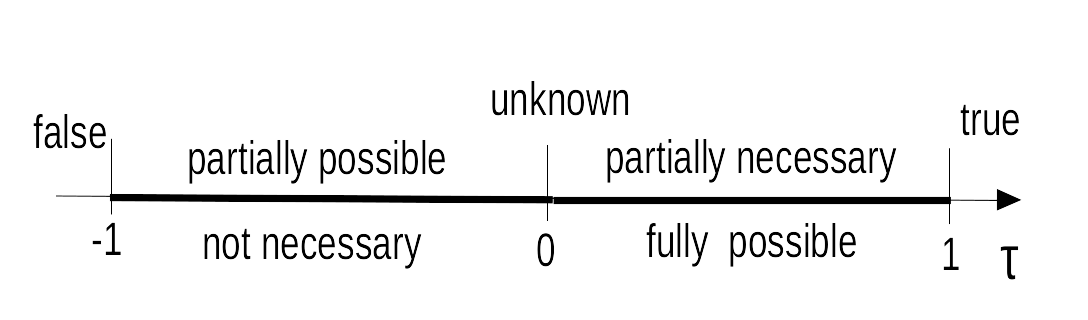
\includegraphics[width=0.5\textwidth]{figures/possibility-necessity.png}}
\caption{Representation of partial truth $\tau \in [-1,1]$, in link with necessity and possibility.}
\label{possibility-necessity}
\end{figure}

As discussed in the introduction, this modal notion of partial knowledge or belief is not only epistemic or doxastic, but also deontic and so on, i.e., has several semantic interpretation, depending on the concept quality. Our strong hypothesis here, is that all modalities can be encoded using the proposed numerical grounding.

We thus now can represent a quantity with a partial degree of belief $\tau \in [-1, 1]$ and uses the notation:
\eqline{\hat{\mathbf{x}} \deq \tau \, \mathbf{x}}
where $\mathbf{x}$ corresponds to the numerical grounding of a symbol, and $\hat{\mathbf{x}}$ the numerical grounding of a symbol weighted by a modality quantification $\tau$, thus of magnitude $O(|\beta|)$.

\subsection{Knowledge structure encoding.}

Let us now review how we can biologically implement symbolic data structure within the proposed framework. This section simply revisits the literature, emphasizing the data structure properties.

\paragraph{Unordered set.} We first consider an unordered set ${\cal S}$ of $N$ symbols grounded to values $\{\mathbf{s}_1, \cdots \mathbf{s}_i \cdots \mathbf{s}_N\}$ and would like to be able to store them, in such a way that we can check if the symbol is in the set. Very simply, we ground ${\cal S}$ to the vector $\mathbf{s}$ :
\eqline{\mathbf{s} \deq \sum_i \mathbf{s}_i}
provides a solution, because given a symbol $\mathbf{s}_\bullet$ we obviously observe that $\mathbf{s}_\bullet \cdot \mathbf{s} \simeq 1$ if it corresponds to one $\mathbf{s}_i$ and almost $0$ otherwise, because random vectors are almost orthogonal as previously explained.

This obviously generalized to weighted symbols $\hat{\mathbf{s}}_i$, i.e., with a modality weighting. In that case $\mathbf{s}_\bullet \cdot \mathbf{s} \simeq \tau$ allows to retrieve the belief weight.

Furthermore, the representation intrinsically includes a notion of transitivity: If a set includes another subset, by construction, its includes the subset elements, more precisely:
\eqline{\mathbf{s} \deq \sum_i \mathbf{s}_i \mbox{ and } \mathbf{s}_i = \deq \sum_j \mathbf{s}_ij \Rightarrow \mathbf{s} \deq \sum_{ij} \mathbf{s}_ij}
thus $\mathbf{s}_{ij} \cdot \mathbf{s} > 0$ for all subsets elements.

This has an interesting biological interpretation: ${\cal S}$ corresponds to neural map, where information has been stored in a distributed way, and activating the map with an input $\mathbf{s}_\bullet$ allows to retrieve if the symbol is stored, or not, in one step. It corresponds to a \vthierry{AJouter ref et preciser}{}.

At this stage, this structure does not allow to directly enumerate all symbols $\mathbf{s}_i$, because from $\mathbf{s}$ it is not possible to decode the superposed vectors. There is no ``select'' operator allowing to select all elements and perform an operation on each one. In \cite{crawford_biologically_2016}, for instance, where data structures are defined using superposition, the memory retrieval of the stored information is not addressed\footnote{However, it seems that at the implementation level, in Nengo \cite{eliasmith_how_2013}, an explicit list of the defined vocabulary $\{\cdots \mathbf{s}_i \cdots\}$ is maintained, and the way to select the elements is to test $(\mathbf{s}^T \, \mathbf{s}_i)$ for each element of the vocabulary. Such select operator complexity is of $O(K)$ where $K$ is the size of the vocabulary. \vthierry{Euh la c est moi qui raconte ca de memoire du une discussion avec Terry ... cest à confirmer}{}}.

\paragraph{Associative map.} We now consider an unordered associative ${\cal M}$ map of $N$ correspondences $\{\mathbf{s}_1 \rightarrow \mathbf{o}_1, \cdots \mathbf{s}_i \rightarrow \mathbf{o}_i \cdots \mathbf{s}_N \rightarrow \mathbf{o}_N\}$ between subjects and objects. To this end, we use binding operation $B_{\mathbf{s}_i}$ with a pseudo inverse, i.e. an unbinding operator, $B_{\tilde{\mathbf{s}}_i}$:
\eqline{\mathbf{m} \deq \sum_n B_{\mathbf{s}_i} \, \mathbf{o}_i}
so that 
\eqline{B_{\tilde{{\mathbf{s}}_\bullet}} \, \mathbf{m} \simeq \sum_{i, \mathbf{s}_\bullet = \mathbf{s}_i} \mathbf{o}_i.}
In words, the unbinding operation allows to retrieve the set, i.e., the additive superposition of all objects $\mathbf{o}_i$ associated to a given subject $\mathbf{s}_\bullet$, while $B_{\tilde{\mathbf{s}}_k} \, {\cal S} \simeq 0$ if none.

This allows to both detect if the information is in the table and retrieve this information in one step, if it the case. However, as in the previous case, no mechanism allows to enumerate the map subjects or objects.

This algebraic construction also allows to retrieve the subjects associated to a given objects, because of commutator $\mathbf{B_{\leftrightarrow}}$ such that
\eqline{\mathbf{B_{\leftrightarrow}} \, \mathbf{B}_{\mathbf{o}_i} \, \mathbf{s}_i = \mathbf{B}_{\mathbf{s}_i} \, \mathbf{o}_i,}
yielding:
\eqline{\mathbf{m_{\leftrightarrow}} \deq \mathbf{B_{\leftrightarrow}} \, \mathbf{m} = \sum_i B_{\mathbf{o}_i} \, \mathbf{s}_i,}
which is now the numerical grounding of the reciprocal map $\{\mathbf{o}_1 \rightarrow \mathbf{s}_1, \cdots \mathbf{o}_i \rightarrow \mathbf{s}_i \cdots \mathbf{o}_N \rightarrow \mathbf{s}_N\}$.

The algebraic system also offers the notion of identity vector $\mathbf{i}$ with $\mathbf{B_{\mathbf{i}}} = \mathbf{I}$ so that:
\eqline{\mathbf{s}_i = \mathbf{i} \rightarrow B_{\mathbf{s}_i} \, \mathbf{o}_i = \mathbf{o}_i}
in other words the binding reduces to a superposition.

Such mechanism does not allow to directly enumerate all subjects stored in the associative memory, as already discussed for the set elements.

This associative memory mechanism has an interesting biological interpretation: ${\cal M}$ corresponds to an associative memory with association storing in a distributed way, and activating the map with an input $\mathbf{s}_\bullet$ allows to retrieve the associated symbol. This is what happens in several biological mechanism \vthierry{Rajouter ref et expliciter}{}.

There are several solutions to define such binding, unbinding and commutator operators. A proposed solution is developed in Appendix~\ref{VTB-algebra} after \cite{gosmann_vector-derived_2019} completed by \cite{mercier_ontology_2021}. This design choice is guided by the fact we need to retrieve \vthierry{Ici je veux bien rediscuter pourquoi on veut pas que ce soit associatif ni commutatif ... j ai besoin d aide}

\paragraph{Indexes for list and iterator.} In order to define indexed list, we need indexes, i.e., a mechanism that generates ordinal values, \vthierry{as developed in for convolution operator citer ref et dire un peu plus, dans generalized here to VTB}{}. We fix the symbol grounding of the ``zero'' symbol $\mathbf{i}_0$ and defines recursively:
\eqline{\mathbf{i}_{n + 1} \deq B_{\mathbf{i}_0} \, \mathbf{i}_n}
i.e. the $(n+1)$-th index value is obtained by binding the $n$-th nd we easily obtain
\eqline{B_{\mathbf{i}_p} \, \mathbf{i}_q = B_{\mathbf{i}_q} \, \mathbf{i}_p = B_{\mathbf{i}_{p+q}}, \;\;\; 
B_{\mathbf{i}_p} \, \tilde{\mathbf{i}}_q = B_{\tilde{\mathbf{i}}_q} \, \mathbf{i}_p  \simeq B_{\mathbf{i}_{p-q}},}
in particular $\mathbf{i}_{n - 1} \simeq B_{\tilde{\mathbf{i}}_0} \, \mathbf{i}_n$ so that the definition holds for $n \in {\cal Z}$.

\paragraph{Indexed list.} We now can define indexed list, or array, often called vector, since the previous mechanism allows us to generates a ``counter'' that could be increment or decremented using the binding or unbinding operator.

Then, an associative map indexed by these ordinals can be managed as a list, which values can be enumerated. Such representation is also present at several cognitive levels, when considering temporal sequences, of actions or of enumeration. This is also the tool that allows is to enumerate all elements of a symbol set ${\cal S}$ previously defined, or the subjects of an associative map.

To make this mechanism explicit, let us consider a list $\mathbf{l} \deq \sum_i B_{\mathbf{i}_i} \, \mathbf{l}_i$, and a variable index $\mathbf{k}$: A construct of the form:
\begin{algorithmic}
\For{$\mathbf{k} \leftarrow \mathbf{i}_0$; {\bf while} $|B_{\mathbf{k}} \, \mathbf{l}| > 0$; {\bf next} $\mathbf{k} \leftarrow B_{\mathbf{i}_0} \, \mathbf{k}$}
   \State $\mathbf{l}_i \leftarrow B_{\tilde{\mathbf{k}}} \, \mathbf{l}$
   \State ../..
\EndFor   
\end{algorithmic}
allows to enumerate\footnote{In fact, considering $\mathbf{l} \deq \sum_i B_{\mathbf{i}_i} \, \mathbf{l}_i + B_{\mathbf{i}_{-1}} \, \lambda$ where $\lambda$ is the list length, updated when adding or deleting an element would improve the algorithmic ersatz implementation, which is not the issue here.} all elements, this being indeed only an algorithmic ersatz to illustrate the mechamism beyond the bioplausible implementation.

\paragraph{Nested associated map and triple store}

Let us now consider we have a set of bean of knowledge of the form of Fig.~\ref{triple}, bounded to a triple of vectors $\{(\mathbf{s}_1 \mathbf{p}_1 \mathbf{o}_1.), \cdots (\mathbf{s}_N \mathbf{p}_N \mathbf{o}_N.)\}$ we first need to store this information in a biological ``triple store'' using superposition, and a few binding operations. The most natural choice might be to consider triple set $\mathcal{S}$ grounded to a vector $\mathbf{s}$ :
\eqline{\mathbf{s} \deq \sum_i \mathbf{B}_{\mathbf{p}_i} \, \mathbf{B}_{\mathbf{s}_i} \, \mathbf{o}_i.}

Here we introduce another algebraic ingredient $\mathbf{B}_{\mathbf{p}_i \oslash \mathbf{s}_i} \deq \mathbf{B}_{\mathbf{p}_i} \, \mathbf{B}_{\mathbf{s}_i}$ defining the combination of two binding operators, as again detailed in Appendix~\ref{VTB-algebra}.

This in fact corresponds to a nested map, with the following interesting properties that
\eqline{\mathbf{m}_{\mathbf{p}_\bullet} \deq  B_{{\mathbf{p}_\bullet^\sim}} \, \mathbf{s} \simeq \sum_{i, \mathbf{p}_\bullet = \mathbf{p}_i} \mathbf{B}_{\mathbf{s}_i} \, \mathbf{o}_i}
corresponds to the associative map for a given predicate $\mathbf{p}_\bullet$.

By further combination:
\eqline{\mathbf{m}_{\mathbf{p}_\bullet, \mathbf{s}_\bullet} \deq \mathbf{B}_{(\mathbf{p}_i \oslash \mathbf{s}_i)^\sim} \, \mathbf{m} = \sum_{\mathbf{p}_\bullet = \mathbf{p}_i, \mathbf{s}_\bullet = \mathbf{s}_i} \mathbf{o}_i}
allows to select by predicate and subject the given objects, while
\eqline{\mathbf{m}_{\mathbf{p}_\bullet, \mathbf{o}_\bullet} \deq 
\mathbf{B}_{\mathbf{o}_\bullet^\sim} \, \mathbf{B_{\leftrightarrow}} \,  \mathbf{B}_{{\mathbf{p}_\bullet^\sim}} \, \mathbf{m} = 
\sum_{\mathbf{p}_\bullet = \mathbf{p}_i, \mathbf{o}_\bullet = \mathbf{o}_i} \mathbf{s}_i}
allows to select by predicate and object the given subjects.

Moreover, an additional symbol ``unknown'', which numerical grounding is fixed to any new random vector $\mathbf{u}$ allows to enhance the information to be obtained. Each time a triplet $(\mathbf{s}_i \mathbf{p}_i \mathbf{o}_i.)$ we also add 
$(\mathbf{u} \mathbf{p}_i \mathbf{o}_i.)$, $(\mathbf{s}_i \mathbf{u} \mathbf{o}_i.)$, $(\mathbf{s}_i \mathbf{p}_i \mathbf{u}.)$. This allows to retrieve the fact that there is a link between predicate and object, subject and object, and subject and predicate, without requiring to enumerate the different elements. This could also be used at the level of a single associative map. \vthierry{Et la il faut ajouter que ``unknown peut mener à de fausses conclusions. Il faut donc projeter tout les vecteurs sur l’orthogonal de unknown quand on ne souhaite pas que unknown joue un rôle.'' mais je sais vachement plus pourquoi ....}{}

At the cognitive level, this corresponds to cognitive maps in interaction. Each map is associated to predicate. The fact maps can be combined in triple stores as made explicit here, eases operations involving between them as developed now.

\vthierry{Ici j envisage meme de parler des structures de donnees comme celles dans le papier dee creativite, voir de dicuter de distance d edition .... ou d une approximation}{}

\subsection{Knowledge transformation encoding.}

At this stage, we have reviewed and completed the Vector Symbolic Architecture (VSA) elements allowing to define symbols and memorize them and relation between them in biologically plausible structures. The next step is to define operators allowing to enrich the memorized information, using biologically plausible transformations.

Here we consider combination of associative maps, or equivalently a triple store.

\paragraph{Basic unary and binary operation.} 

Let us write:
\eqline{(\mathbf{\$s}_0 \; \tau_0 \, \mathbf{\$p}_0 \; \mathbf{\$o}_0 .)}
the fact that a variable subject $\mathbf{\$s}_0$ is associated to a variable object $\mathbf{\$o}_0$ in an associative table related to predicate variable $\mathbf{\$p}_0$ with a level of belief $\tau_0$, i.e.:
\eqline{\mathbf{m}_{\mathbf{\$p}_0} = \tau_0 \, \mathbf{B}_{\mathbf{\$s}_0} \, \mathbf{\$o}_0 + \cdots,}
considering as discussed before the knowledge representation structure as a set of associative maps in interaction.

In our context we consider operations of the form:
\eqline{(\mathbf{\$s}_1 \; \mathbf{\$p}_1 \; \mathbf{\$o}_1 .) \mbox{ and } (\mathbf{\$s}_2 \; \mathbf{\$p}_2 \; \mathbf{\$o}_2 .) \Rightarrow (\mathbf{\$s}_0 \; \tau_0 \, \mathbf{\$p}_0 \; \mathbf{\$o}_0 .)}
or
\eqline{(\mathbf{\$s}_1 \; \mathbf{\$p}_1 \; \mathbf{\$o}_1 .) \Rightarrow (\mathbf{\$s}_0 \; \tau_0 \, \mathbf{\$p}_0 \; \mathbf{\$o}_0 .)}
with one premise or a conjunction of two premises yielding a new element which right-hand values are obtained from left-hand side elements, mainly considering equality constraints.

Let us immediately consider an example.

\paragraph{The basic class inheritance rule example.}
\vthierry{Reprendre en nettoyant les vocables RDFs mais juste isa …}

The most common entailment rule is likely the class inheritance rule, which states that ``if a subject belongs to a class, and if this class is a subset of a super class, then the subject belongs to the super class'', e.g., ``if Tom is a cat, and cat are animals, then Tom is an animal''. Let us write this rule, considering the RDFS vocabulary, as discussed in Appendix~\ref{RDFS-entailment-rules}:
\eqline{(\mathbf{\$s} \; \texttt{\bf rdf:type} \; \mathbf{\$c}_1 .) \mbox{ and } (\mathbf{\$c}_1 \; \texttt{\bf rdfs:subClassOf} \; \mathbf{\$c}_2 .) \Rightarrow (\mathbf{\$s} \; \texttt{\bf rdf:type} \; \mathbf{\$c}_2 .)}
that states that if any subject $\$s$ belongs to the class $\mathbf{\$c}_1$, i.e., is of ``type'' $\mathbf{\$c}_1$, and this class $\mathbf{\$c}_1$ is a subclass of $\mathbf{\$c}_2$, then $\mathbf{\$s}$ also belongs to the class $\mathbf{\$c}_2$.

If we consider the forward implementation of the previous mechanism, i.e., given two left-hand side triples, numerically calculates the right-hand side. To this end, we need to consider the similarity operator $(\mathbf{x} \cdot \mathbf{y})$ and a numerical implementation of the conjunction $(\mathbf{x} \And \cdots \And \mathbf{y})$ operator, equals to:
\\ \tab \tab - $0$ as soon one operand is equal or less than $0$, 
\\ \tab \tab - $1$ if all operand equal $1$,
with intermediate values if operands are between $0$ and $1$. This could simply be a product or a $\min$ operator \vthierry{Je laisse le choix ouvert à ce stade on a des elements qq part pour en discuter plus, à voir.}{}.

Then the class inheritance application rule can be written, as schematized in Fig.~\ref{rdfs9-derivation}:
\eqline{(\mathbf{\$s}_1 \; \mathbf{\$p}_1 \; \mathbf{\$o}_1 .) \mbox{ and } (\mathbf{\$s}_2 \; \mathbf{\$p}_2 \; \mathbf{\$o}_2 .) \Rightarrow (\mathbf{\$s}_1, \tau \, \texttt{\bf rdf:type}, \mathbf{\$o}_2)}
with 
\eqline{\tau \deq (\mathbf{\$p}_1 \cdot \texttt{\bf rdf:type}) \And (\mathbf{\$o}_1 \cdot \mathbf{\$s}_2) \And (\mathbf{\$p}_2 \cdot \texttt{\bf rdfs:subClassOf}),}
so that $\tau$ equals $0$ unless the three equalities are verified. If equals to $0$ nothing is inferred, whereas if higher than $0$, a new triple is output. It is a forward schema in the sense that given some input data, a new result is inferred.

\begin{figure}[ht]
 \centerline{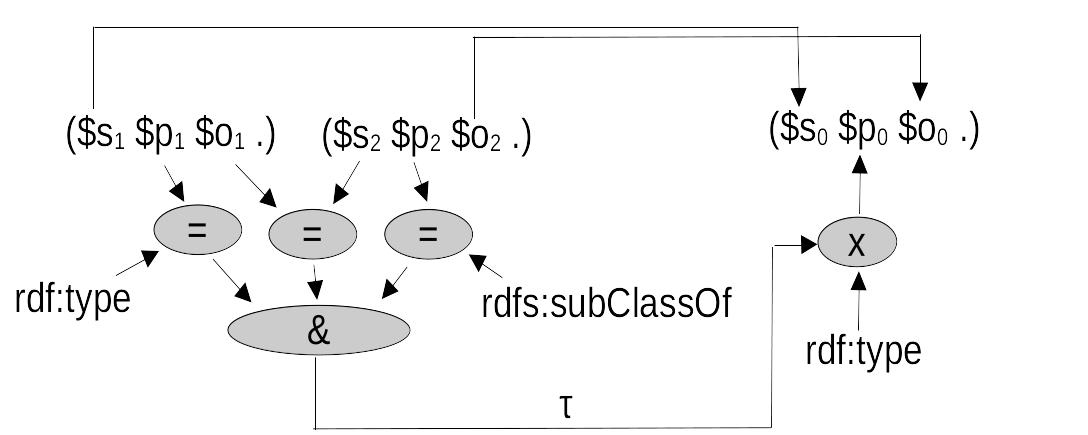
\includegraphics[width=0.75\textwidth]{figures/rdfs9-derivation.png}}
 \caption{The implementation of the class inheritance entailment rule.}
 \label{rdfs9-derivation}
\end{figure}

We may also consider the backward implementation of this rule, i.e., given a triplet of the form $(\mathbf{\$s}_0 \; \tau_0 \, \mathbf{\$p}_0 \; \mathbf{\$o}_0 .)$, with some of the variable optionally similar to a vector of the vocabulary, perform a recurrent backward search of left-hand side compatible triples, so that applying the rule generates a triple compatible and similar with the given right-hand side one, see e.g., \cite{kapoor_comparative_2016} for an overview. This will be further discussed in the next section.

\paragraph{Implementation of approximate inference.} Interesting enough, this rule is still valid when considering approximate similarity: If the input triple states that $\textbf{\$s}_1$ is approximately of class $\textbf{\$o}_1$, with $\textbf{\$p}_1 = \tau \, \texttt{\bf rdf:type}$, with $\tau \in [0,1]$, and similar approximate equalities, while the similarity operator outputs a value between 0 and 1 and the conjunction operators interpolate values between $0$ and $1$ given the input, we will obtain as output an appropriate predicate value $\tau' \, \texttt{\bf rdf:type}$, with $\tau' \in [0,1]$, which corresponds to the fact the predicate is only approximately true.

\paragraph{Implementation of negative inference.} This however does not immediately generalize to negative inference (i.e., the fact it approximately does {\em not} belong to a given class, which is beyond RDFS specification but present at the OWL level), but sill : In that case, a symmetric rule: 
\eqline{(\mathbf{\$s} \; \neg \texttt{\bf rdf:type} \; \mathbf{\$c}_1 .) \mbox{ and } (\mathbf{\$c}_2 \; \texttt{\bf rdfs:subClassOf} \; \mathbf{\$c}_2 .)  \Rightarrow (\mathbf{\$s} \; \neg \texttt{\bf rdf:type} \; \mathbf{\$c}_2 .)}
has to be considered, with a totally similar development. The key point, here, is that we must only consider positive part of the similarity, i.e., combine with a rectification operator.

\vthierry{Ici ajouter les deux mechansimes closure ou request}

\paragraph{More general mechanisms.} Beyond this class inheritance rule example, the proposed unary or binary rules mechanisms allows to infer what can be logically deduced from the input information. In Appendix~\ref{RDFS-entailment-rules}, we make explicit the fact that a very commonly used Semantic Web modeling languages, the RDFS (Resource Description Framework Schema) can have its main mechanisms implemented in such a numerical framework, while in \cite{mercier_ontology_2021}, which have introduced this idea it is also shown that some OWL (Web Ontology Language) construction are also implementable.
A step further, it must be noticed that the proposed rules do not restrain to such logical deduction, but may also integrate quantitative evaluation (e.g., with explicit computations of some expression). With different rules format, but the same approach, not only deduction, but also rule-based induction \cite{domingos_unifying_1996} or rule-based abduction mechanisms \cite{lakkaraju_rule_2000}, could be also considered as a perspective of this work. 

\paragraph{Entailment mechanisms.} Given such rules, the next step is to define entailment, i.e., all what can be logically deduced from the input information, can be realized. In the brain, as discussed for instance in \cite{oreilly_goal-driven_2014} at a computational level and \cite{friston_learning_2003} at a more conceptual level, both forward and backward mechanisms are mixed in cognitive behaviors, as studied for instance in \cite{amidu_protocol_2019} at a more experimental level.

In a nutshell, entailment rules are applied both ``on query'' when, given a goal-directed behavior, some information is required and at a more data-driven level, here stimulus-driven level, when a new input is not only to be memorized but also processed \cite{kapoor_comparative_2016}. 

In both cases, given the data structures considered here, in both forward and backward cases, the key issue is the enumeration of all appropriate triples in order to check to what extents they correspond to the rule. This is made explicit in Appendix~\ref{RDFS-entailment-rules-1} for the class inheritance rule example.

\vthierry{Bon je m arrete la .. c est tres preliminaire mais ca donne une idee de ce que je te propose de faire ...}

\subsection{Implementation at the macroscopic scale}

This Vector Symbolic Architecture (VSA) when implemented using the Neural Engineering Framework (NEF) allows a microscopic simulation of the neuronal processes, at the spiking neural network level, of the memorization and processing operations, for which we have developed an abstract symbolic description previously. At a higher scale, when implemented as described in Appendix~\ref{VTB-algebra} using linear algebra and permutation operations, we are at a mesoscopic scale allowing to perform the same operations, but without explicitizing the neural state value and evolution. This is one major advantage of this class of approaches.

Here we propose, at a higher macroscopic scale, to directly consider the previous operations predicting the result of the different algebraic operations without explicitly working at the vector component level. Let describe how this can be designed and implemented, using what could be called an ``algorithmic ersatz''.

\paragraph{Symbol indexing.} In VSA, each symbol of the vocabulary is associated to a $d$-dimensional random vector. At the macroscopic scale we only need to register each symbol by an index, incremented for each new symbol. Weighted symbols have also a ``belief'' value $\tau$ as discussed previously, equal to $1$ by default. Two symbols my thus have the same index but with a different belief level. At the input/output level, only, a human readable string representation of the symbol is associated. The ``symbol'' table is thus simple array data structure, with an index, a weight and a string.

The similarity operation between two symbols is calculated from the index table, without explicitly computing a dot-product. Given a dimension $d$, the result for two symbols with different indexes is $\nu \simeq {\cal N}(0, O(1/d))$ i.e., almost zero, up to a normal noise. For two weighted symbols of entry $i$ and $j$ with the same index, the value is calculated from their weight $\nu \simeq {\cal N}(\tau_i\,\tau_j, O(1/d))$. This design choice introduces a crucial difference with the mesoscopic implementation: If the symbol numerical random vectors are drawn once, their dot-products will be defined up to a certain level of noise, but defined once. Here, at each dot-product value calculation, the additive noise value is re-drawn. We consider that it is more realistic than a freezed noise value, although it would have been easy to consider freezed noise values and cache them in some table.

In our context, additional compounded symbols are defined by either superposition, or binding and combination of binding operations, while similarity has to be computed on any of these compounded symbols. A the macroscopic level it is straightforward to define an ``oracle'' that can calculate the result of all operations, as follows.

At the compounded symbols specification level:
\\- A symbol corresponding to the {\em superposition} of other symbols is fully defined by the symbol set.
\\- A symbol corresponding to the {\em binding} of one symbol onto another is fully defined by the symbols pair.
\\- A symbol implied in {\em unbinding} corresponds is fully defined by the symbol it is the inverse of.
\\- A symbol corresponding to the {\em combination} of two binding operations (the $\oslash$ operator) is fully defined by the symbol pair.

At the algebraic operation level, since we use linear algebra as detailed in appendix~\ref{VTB-algebra}, it is rather straightforward to predict the result of any operations, up to some additive noise:
\\ Operation over a superposition (binding or similarity) results of applying the operation on each element and consider either the superposition (in the case of binding) or numerical sum (in the case of similarity) of the result.
\\ Operation over a binding yields either to a reduction if it is the corresponding unbinding operation or a binding combination.
\\ While we obtain similar mechanisms for, e.g., the commutator operator $\mathbf{B_{\leftrightarrow}}$.

\vthierry{Je propose que tu prennes connaissance de cette idée et si ok on pourrait s amuser à ecrire les règles à appliquer dans un langage à choisir ensemble de maple à un langage impératif facile à utiliser}

\bibliographystyle{apalike}
\bibliography{AIDE}

\appendix

\section{Using the VTB algebra} \label{VTB-algebra}

Symbols are numerical grounding to real or complex vectors of quartic dimension $d = (d'')^4$ for some integer $d''$. Let us develop here the algebra to manipulate such symbols at an abstract level. Following \cite{gosmann_vector-derived_2019} and completing their developments, we consider biologically a plausible algebraic framework, each numerical grounding corresponding to some distributed  activity of a spiking neuronal assemble and each algebraic operation to some transformation of this activity.

\vthierry{Creer code de verif: gerer matrice, comparer les deux calculs}

We first consider the so called Vector-derived Transformation (VTB) binding operation:
\eqline{\mathbf{z} = \mathbf{B_y} \, \mathbf{x}}
where $\mathbf{B_y}$ is block-diagonal matrix defined as, writing $d' \deq \sqrt{d}$:
\eqline{\mathbf{B_y} \deq 
\left[\begin{array}{cccc}
    \mathbf{B_y'} &    0 & \dots &   0 \\
       0 & \mathbf{B_y'} & \dots &    0 \\
    \vdots & \vdots & \ddots & \vdots  \\
       0 &    0 & \dots & \mathbf{B_y'}
    \end{array}\right]
\mbox{ with } 
\mathbf{B_y'}  \deq  \sqrt{d'} \,
\left[\begin{array}{cccc}
    y_1            & y_2            & \dots  & y_{d'}  \\
    y_{d' + 1}     & y_{d' + 2}     & \dots  & y_{2d'} \\
    \vdots         & \vdots         & \ddots & \vdots  \\
    y_{d - d' + 1} & y_{d - d' + 2} & \dots  & y_d
\end{array}\right]}
or equivalently, for $i = 1 \cdots d$:
\eqline{[\mathbf{z}]_i = \sqrt{d'} \, \sum_{k = 1}^{i = d'} [\mathbf{y}]_{k + d' \, ((i-1) \mbox{ mod } d')} \;
[\mathbf{x}]_{k + d' \, ((i-1) \mbox{ div } d')}}
with the matrix multiplication explicitized as a sum, as it can be easily verified. Here $[\mathbf{z}]_k$ stands for the k-th coordinate of the vector $\mathbf{z}$.

This operation is bi-linear in $\mathbf{x}$ and $\mathbf{y}$, thus distributive with respect to addition.

At the algorithmic implementation level, the calculation is performed in $O\left(d^{\frac{3}{2}}\right)$ operations, and the $\mathbf{y}_{k + \beta[i]}$ and $\mathbf{x}_{k + \alpha[i]}$ indexing can be tabulated in two fixed look-up tables $\beta[i]$ and $\alpha[i]$ avoiding any additional calculations. Furthermore, the fact that $\sqrt{d'}$ is an integer allows to limit numerical approximations in order to improve the numerical conditioning.

As stated in \cite{gosmann_vector-derived_2019} and reviewed in \cite{mercier_ontology_2021} the key point is that this binding operation generates a new vector $\mathbf{z}$ almost orthogonal to $\mathbf{x}$ and $\mathbf{y}$ and this operation is neither commutative nor associative, i.e.:
\eqline{(\mathbf{B_y} \, \mathbf{x}) \cdot \mathbf{x} \simeq 0 \mbox{ and } (\mathbf{B_y} \, \mathbf{x}) \cdot \mathbf{y} \simeq 0 \mbox{ and } (\mathbf{B_x} \, \mathbf{y}) \cdot (\mathbf{B_y} \, \mathbf{x}) \simeq 0 \mbox{ and } (\mathbf{B_{B_z \, y}} \, \mathbf{x}) \cdot ((\mathbf{B_z} \, \mathbf{B_y}) \, \mathbf{x}) \simeq 0}
which are precious properties in order not to infer spurious derivations. These results come from the fact that these vectors pairs are not aligned but have an orientation parameterized by random vectors. More precisely, two random normalized vectors drawn from a random normal distribution of independent samples verify ${\bf x} \cdot {\bf y} \sim {\mathcal N}(0, O(1/d))$, i.e., follows a centered normal distribution of negligible variance \cite{schlegel_comparison_2020}. A step ahead, when computing $\mathbf{B_y} \, \mathbf{x}$ we apply a permutation on all indices so that the result is no more correlated with the original vectors, thus corresponding to independent values, and leading also to almost zero.
% Beuh c'est pas très rigoureux mais bon on écrit les équations on finit par faire la même hypothèse "morale".

\vthierry{Remplacer les $\sim$ par des tilde partout}

A step further, in the real case, the random matrix is almost orthogonal, i.e.:
\eqline{\mathbf{B_y^\top} \, \mathbf{B_y} \simeq \mathbf{I}}
for the same reasons evoked just before. We thus can defined:
\eqline{\mathbf{B_{y^\sim}} \deq \mathbf{B_y^\top} \mbox{ with } [\mathbf{y^\sim}]_i \deq [\mathbf{y}]_{\sigma(i)} \mbox{ and }  \sigma(i) \deq  1 + d' \, ((i-1) \mbox{ mod } d') + (i-1) \mbox{ div } d'}
in words $\mathbf{B_y^\top}$ has the same structure as $\mathbf{B_y}$ except that the vector coordinates are subject to a permutation $\sigma(i)$ which is idempotent $\sigma(\sigma(i)) = i$, thus its own inverse, so that if 
$\mathbf{z'} = \mathbf{B_{y^\sim}} \, \mathbf{x}$ we obtain:
\eqline{[\mathbf{z'}]_i = \sqrt{d'} \, \sum_{k = 1}^{k = d'} [\mathbf{y}]_{\sigma(k + \beta(i))} \; [\mathbf{x}]_{(k + \alpha(i))}} (where $\beta(i)$ and $\alpha(i)$ are the indexing defined to calculate $\mathbf{B_{y}} \, \mathbf{x}$ explicitly) and it allows to define a left unbinding operation:
\eqline{\mathbf{B_{y^\sim}} \, (\mathbf{B_y} \, \mathbf{x}) = \mathbf{B_y^\top} \, \mathbf{B_y} \, \mathbf{x} \simeq \mathbf{x}}

\vthierry{Virer les alpha beta et mettre formule explicite ou bien les definir}

The right identity vector $\mathbf{\mathbf{i}}$ such that $\mathbf{B_{\mathbf{i}}} = \mathbf{I}$, writes explicitly:
\iftrue
\eqline{[\mathbf{\mathbf{i}}]_i = \frac{1}{\sqrt{d'}} \, \delta_{i = \sigma(i)}}
In other words, we get $i_B$ by ``unfolding'' the identity matrix $I_d'$ line by line, writing a $1$, then $d$ times $0$, another $1$, and so on.
\else
\eqline{\mathbf{\mathbf{i}} \deq \frac{1}{\sqrt{d'}} \, \left(1, \underbrace{0, \cdots 0}_{d' \mbox{\scriptsize times}}, 1, \underbrace{0, \cdots 0}_{d' \mbox{\scriptsize times}}, 1, \cdots, 1\right)^T.}
In other words, we get $i_B$ by ``unfolding'' the identity matrix $I_d'$ line by line, i.e., the $i$-th coordinate is zero unless $i = (k - 1) \, d' + k$ for some $k, 0 < k \leq d'$, which also corresponds to $i = \sigma(i)$.
\fi

Considering the mirroring matrix $\mathbf{B_{\leftrightarrow}}$ defined as:
\eqline{[\mathbf{B_{\leftrightarrow}}]_{ij} \deq \delta_{j = \sigma(i)}}
(with is thus not block-diagonal as matrix of the form $\mathbf{B_y}$ are) we obtain:
\eqline{\mathbf{B_{\leftrightarrow}} \, \mathbf{B_y} \, \mathbf{x} = \mathbf{B_x} \, \mathbf{y}
\mbox{ while } \mathbf{B_{\leftrightarrow}} \,\mathbf{B_{\leftrightarrow}} = \mathbf{I} \mbox{ and } \mathbf{B_{\leftrightarrow}^\top} = \mathbf{B_{\leftrightarrow}}.}
which allows to define a right unbinding operation:
\eqline{(\mathbf{B_{x^\sim}} \, \mathbf{B_{\leftrightarrow}}) \, (\mathbf{B_y} \, \mathbf{x}) = \mathbf{B_{x^\sim}} \, \mathbf{B_x} \, \mathbf{y} \simeq \mathbf{y}}

\vthierry{Expliciter $[\mathbf{z}'']_i = \mathbf{B_{\leftrightarrow}}) \, \mathbf{x}$ avec les indexes}

Unfortunately $\mathbf{B_{\leftrightarrow}}$ is not a binding matrix, i.e., is not of the form $\mathbf{B_z}$ for some vector $\mathbf{z}$, and the left or right multiplication of a binding matrix by this mirroring matrix does not yield a binding matrix. However, the calculation $\mathbf{w} = \mathbf{B_{x^\sim}} \, \mathbf{B_{\leftrightarrow}} \, \mathbf{z}$ can be made explicit yielding:
\eqline{[\mathbf{w}]_i = \sqrt{d'} \, \sum_{k = 1}^{k = d'} [\mathbf{x}]_{??} \; [\mathbf{z}]_{???}}
\vthierry{CE QUI RESTE A FAIRE !}

\vthierry{Remplacer w par z'''}

Beyond \cite{gosmann_vector-derived_2019}, \cite{mercier_ontology_2021} has introduced a vector composition operator $\oslash$ making explicit the composition of two binding operations, namely:
\eqline{\mathbf{B_v} = \mathbf{B_y} \, \mathbf{B_x} \Leftrightarrow \mathbf{v} \deq \mathbf{y} \oslash \mathbf{x}}
which explicitly writes:
\eqline{[\mathbf{v}]_i = \sqrt{d'} \, \sum_{k = 1}^{k = d'} [\mathbf{y}]_{k + (i - 1) \mbox{ div } d'} \; [\mathbf{x}]_{1 + d' \, (k - 1) + (i - 1) \mbox{ mod } d'}}
as obtained explicitizing that $\mathbf{B_v}' = \sqrt{d'} \,\mathbf{B_y}' \, \mathbf{B_x}'$ using the notation of the first definition. The key point is that the product of two binding matrices is still a binding matrix. As a consequence this composition operator is bi-linear, thus distributive with respect to the addition, it is not commutative, but is associative, and commute with the inversion as follows:
\eqline{(\mathbf{y} \oslash \mathbf{x})^\sim = \mathbf{x}^\sim \oslash \mathbf{y}^\sim}
while $\mathbf{x}^\sim \oslash \mathbf{x} \simeq \mathbf{\mathbf{i}}$, all these results being easily derived considering usual matrix properties. This allows to combine two binding matrix without explicit matrix product, but also in $O\left(d^{\frac{3}{2}}\right)$ operations only.

\paragraph{Using the VTB algebra in the complex case.}

All developments of this section scale to to complex numbers, which could be an interesting perspective, even if not used here. This could be an interesting perspective.

Stating that two resources are semantically equivalent if the unary vectors are aligned writes in the complex case\footnote{If we are in the real case $\mathbf{x}$ and $\mathbf{y} \in {\mathcal R}^d$, with $\|{\bf x}\|_2 = \|{\bf y}\|_2 = 1$, then the equality writes
\eqline{\mathbf{x} = \mathbf{y} \Leftrightarrow \mathbf{x} \cdot \mathbf{y} = \sum_i x_i \, y_i = \cos\left(\widehat{\overrightarrow{\mathbf{x}} \, \overrightarrow{\mathbf{y}}}\right) = 1 \Leftrightarrow \widehat{\overrightarrow{\mathbf{x}} \, \overrightarrow{\mathbf{y}}} = 0 \; (\mbox{mod} \; 2 \, \Pi),}
i.e., both unary vectors have the same direction, i.e., are aligned.
If we are in the complex case $\mathbf{x}$ and $\mathbf{y} \in {\mathcal C}^d$, let us consider the canonical embedding in ${\mathcal R}^{2\,d}$, i.e., the real $Re$ and imaginary $Im$ parts as two real coordinates, writing $\overrightarrow{\mathbf{x}}$ the corresponding vector:
\eqline{\mathbf{x} \deq \left(x_1, x_2, \cdots \right)^T \Leftrightarrow \overrightarrow{\mathbf{x}} \deq \left(Re(x_1), Im(x_1), Re(x_2), Im(x_2), \cdots\right)^T,}
for which, writing $z^*$ the conjugate of a complex number $z$:
\eqline{\begin{array}{rcl}<\mathbf{x} | \mathbf{y}> 
&\deq& \sum_i x_i \, y_i^* \\
&=& \sum_i 
  (Re(x_i) \, Re(y_i) + Im(x_i) \, Im(y_i)) + I \, (Re(x_i) \, Im(y_i) - Im(x_i) \, Re(y_i)) \\
&=&
  \overrightarrow{\mathbf{x}} \cdot \overrightarrow{\mathbf{y}} + I \, 
  \overrightarrow{\mathbf{x}}^* \cdot \overrightarrow{\mathbf{y}}
\end{array}}
so that $Re(<\mathbf{x} | \mathbf{y}>) = \overrightarrow{\mathbf{x}} \cdot \overrightarrow{\mathbf{y}}$, $\|\mathbf{x}\| = \sqrt{<\mathbf{x}|\mathbf{x}>} = \|\overrightarrow{\mathbf{x}}\|-2 = \sqrt{\overrightarrow{\mathbf{x}} \cdot \overrightarrow{\mathbf{x}}}$ and since vectors are unary: 
\eqline{<\mathbf{x} | \mathbf{y}> = 1 \Leftrightarrow \overrightarrow{\mathbf{x}} \cdot \overrightarrow{\mathbf{y}} = 1 \Leftrightarrow \overrightarrow{\mathbf{x}} = \overrightarrow{\mathbf{y}} \Leftrightarrow \mathbf{x} = \mathbf{y},}

\vthierry{Where $<\mathbf{x} | \mathbf{y}>$ stands for .. expliciter}

making explicit the obvious fact that unary real or complex vectors are equal if and only if their inner product equals one, while we consider the ``angle'' of two complex vectors as the angle of their $2\,d$ real embedding, i.e.:
\eqline{\widehat{\mathbf{x} \, \mathbf{y}} \deq \mbox{arccos}(Re(<\mathbf{x} | \mathbf{y}>)).}}: 
\eqline{\mathbf{x} \simeq \mathbf{y} \Leftrightarrow <\mathbf{x} | \mathbf{y}> \simeq 1.
% https://mathcs.clarku.edu/~ma130/inner2.pdf
} while the orientation is usually defined as:
\eqline{\widehat{\mathbf{x} \, \mathbf{y}} \deq \mbox{arccos}(Re(<\mathbf{x} | \mathbf{y}>)).}
as detailed in the previous footnote.

Provided that the space dimension $d$ is large enough, two randomly chosen different complex vectors $\mathbf{x}$ and $\mathbf{y}$, will be also\footnote{
Considering again the canonical embedding in ${\mathcal R}^{2\,d}$ and the fact that
\eqline{<\mathbf{x} | \mathbf{y}> = \overrightarrow{\mathbf{x}} \cdot \overrightarrow{\mathbf{y}} + I \, 
  \overrightarrow{\mathbf{x}^*} \cdot \overrightarrow{\mathbf{y}},}
because $\overrightarrow{\mathbf{x}}$ thus $\overrightarrow{\mathbf{x}}^*$ and $\overrightarrow{\mathbf{y}}$ are random vectors their dot product almost vanishes, thus the real and imaginary part of $<\mathbf{x} | \mathbf{y}>$ also.} approximately orthogonal in the sense that:
\eqline{\mathbf{x} \neq \mathbf{y} \Leftrightarrow <\mathbf{x} | \mathbf{y}> \simeq 0.}
As a consequence, the VTB matrix is almost a unitary matrix, i.e., 
\eqline{\mathbf{B_y}^* \, \mathbf{B_y} \simeq \mathbf{I}}
considering now the conjugate transpose.

All other algebraic operations are common to both real or complex linear algebra, and this to also the case for other VSA binding operators.

More than a confirmation, these derivations allows us to observe that using a complex representation would be interesting if the conjugate of a vector could be have a semantic interpretation. In that case if, say, $\mathbf{x}$ and $\mathbf{y}^*$ are similar then $<\mathbf{x} | \mathbf{y}> \simeq I$, as easily verified from the previous development. 



\section{RDFS entailment rules numerical implementation} \label{RDFS-entailment-rules}

Considering knowledge representation and reasoning, the capabilities of Semantic Web modeling languages, such as RDFS (Resource Description Framework Schema) and OWL (Web Ontology Language) (see, e.g. \cite{allemang_semantic_2020} for a recent didactic reference) is a powerful way of solving modeling problem and manipulate high-level data representation. It appears also to be rather accessible to educated person, as pointed out in \cite{allemang_semantic_2020}, and corresponds for a certain part to usual common sense formalization, for instance the notion of class (e.g., Garfield is a cat, that is an animal, that is a living organism). The brain is capable of such reasoning, as discussed in the paper introduction, through the data representation and processing mechanism is obviously different from what is performed in semantic web modeler and reasoners, while the brain is mainly doing induction and abduction, more than deduction. However, we would like to show here that our biologically plausible mechanism is at least able to perform RDFS\footnote{According to the \url{ https://www.w3.org/TR/rdf-schema} specification.} specification inferences.

\subsection*{The RDFS modeling in a nutshell}

In order to represent symbolic information the RDFS knowledge representation is based on the RDF data model, which represent knowledge  as triples, as made explicit, in Fig.~\ref{triple}. More precisely, the \emph{universe of discourse} is made of \emph{resources}, referenced by some universal resource identifier (IRI), i.e. a fixed lexical token. To structure this universe of discourse, we consider: \begin{enumerate}[label=(\roman*)]
    \item \emph{individuals} that refer to real-world concrete or abstract objects, or 
    \item \emph{literals} to characterize individuals using data attributes, i.e., numerical values, character strings, or any structured information such as dates
    \item \emph{concepts} and \emph{roles} (namely \emph{classes} and \emph{properties}) that allow to structure the knowledge about individuals.
\end{enumerate}

In fact, in our context which is outside the web semantic application field, we have to point out that the RDF/RDFS framework, has to be considered with the following variants:
\begin{itemize}
    \item we conflate \emph{name} with both IRI and blank node, since on the one hand blank node can be eliminated,\footnote{Using a standard process related to skolemisation.} and on the other hand because we only process the information locally at this stage, thus avoiding considering all issues regarding distributed information between different sources;
    \item we do not consider (i) semantic web specific literal (e.g., \texttt{rdf:XMLLiteral}), or (ii) utility and annotation or other human targeted  properties (e.g., \texttt{rdfs:seeAlso}) at this stage;
    \item we will introduce both containers, i.e., ordered or unordered sequences, and collections, i.e., chained lists, later in these specifications, but in a somehow different form, adapted to the numerical representation and obvious to map on RDF representations;
    \item we do not consider all XSD datatype, but will introduce a precise notion of numerical values and will detail how to represent structured data in our framework.
\end{itemize}

Given the capability of stating facts, the RDFS framework allows to structure the concepts, using the following construct:
\\ - The notion of class inheritance (e.g., if Tom is a cat, and cat are animal, Tom is an animal), which allows to define a hierarchical taxonomy of classes, and structure the objects in categories, and infer all what is possible from this taxonomy.
\\ - The notion of property inheritance (e.g., if Tom is the brother of Jerry, Tom is in the same family as Jerry, the property of being in the same family being a super-property of being the brother), which allows to structure properties, and also infer new properties by inheritance.
\\ - The notion of domain and range (e.g, if Tom is the brother of Jerry, it also means that Tom is a boy), that allows classes for subjects and/or objects of category.

The language also allows to define additional information, such as human readable elements, but we consider as a demonstrative subset to consider the main notions reviewed here.

\subsection{Algorithmic and numeric entailment rule implementation} \label{RDFS-entailment-rules-1}

Let us start considering the class inheritance rule example, defined in the main text which states that ``if a subject belongs to a class, and if this class is a subset of a super class, then the subject belongs to the super class'', e.g., ``if Tom is a cat, and cat are animals, then Tom is an animal''. 

Given two input triples $(\$s_1 \; \$p_1 \; \$o_1 .)$ and $(\$s_2 \; \$p_2 \; \$o_2 .)$, the algorithmic rule forward application writes:
\begin{algorithmic}
\State \textbf{input} $(\$s_1 \; \$p_1 \; \$o_1 .)$ and $(\$s_2 \; \$p_2 \; \$o_2 .)$
\If {$\$p_1 = \texttt{rdf:type} \And \$p_2 = \texttt{rdfs:subClassOf} \And \$o_1 = \$s_2$}
    \State \textbf{output} $(\$s_1 \; \texttt{rdf:type} \; \$o_2 .)$
\EndIf
\end{algorithmic}

Let us now consider a mechanism that incrementally generates all deductions given this rule and incoming triples.

To generate such a closure an efficient mechanism must be able to select the pertinent triples to consider. For instance let us consider that triples are indexed in an associative table by property and subject, i.e., that for two constant values $c_i$, $c_j$:
\begin{algorithmic}
  \State \textbf{select} $(\$s_i \; \$p_i \; \$o_i .), \$p_i = c_i \And \$s_i = c_j$
\end{algorithmic}
can be enumerated directly without scanning all triples but the one to be selected, and that we have the similar efficient associative indexing by property and object. This will allow us to incrementally efficiently calculates the closure as follows, given a ``closed'' set of triples $\{(\$s_i \; \$p_i \; \$o_i .) \cdots \}$ with all possible triplets generated and a new triple $(\$s_0 \; \$p_0 \; \$o_0 .)$ to be added:
\begin{algorithmic}
\State \textbf{input} A new triple $(\$s_0 \; \$p_0 \; \$o_0 .)$ and a closed set of triples $\{(\$s_i \; \$p_i \; \$o_i .) \cdots \}$.
\State \textbf{let} $\{(\$s_0 \; \$p_0 \; \$o_0 .)\}$ an ``open'' triple set, initialized with the new triple inside.
\Repeat
  \State \textbf{pull} a triple $(\$s_0 \; \$p_0 \; \$o_0 .)$ from the open triple set.
  \If{$\$p_0 = \texttt{rdf:type}$}
    \ForAll{$(\$s_i \; \$p_i \; \$o_i .), \$p_i = \texttt{rdfs:subClassOf} \And \$s_i = \$o_0,$ in the closed triple set}
      \State \textbf{add} $(\$s_0 \; \texttt{rdf:type} \; \$o_i .)$ to the open triple set.
    \EndFor
  \ElsIf{$\$p_0 = \texttt{rdf:subClassOf}$}
    \ForAll{$(\$s_i \; \$p_i \; \$o_i .), \$p_i = \texttt{rdf:type} \And \$o_i = \$s_0,$ in the closed triple set}
      \State \textbf{add} $(\$s_i \; \texttt{rdf:type} \; \$o_0 .)$ to the open triple set.
    \EndFor
  \EndIf
  \State \textbf{add} the triple $(\$s_0 \; \$p_0 \; \$o_0 .)$ to the closed triple set.
\Until{the open triple set is empty}
\end{algorithmic}

\subsection{Generality of numeric entailment rule implementation} \label{RDFS-entailment-rules-2}

The RDFS entailment, i.e., all what can be logically deduced from the input information, defines which elements are well-formed and which entailment relations allows to deduced all derived information. In the case of RDFS it is given in Table~\ref{rdfs-entailment-rules}. It appears that each rule can be implemented with the same mechanism, for instance:

- The \textit{rdfs9}  class inheritance entailment rule:
\eqline{(\$s \; \texttt{rdf:type} \; \$c_1 .) \mbox{ and } (\$c_1 \; \texttt{rdfs:subClassOf} \; \$c_2 .) \Rightarrow (\$s \; \texttt{rdf:type} \; \$c_2 .)}
that states that if any subject $\$s$ belongs to the class $\$c_1$ and this class $\$c_1$ is a subclass of $\$c_2$, then $\$s$ also belongs to the class $\$c_2$, as taken as major example here.

- The \textit{rdfs2} rule allowing to infer the subject domain class:
\eqline{(\$s_1 \; \$p_1 \; \$o_1 .) \mbox{ and } (\$p_1 \; \texttt{rdfs:domain} \; \$o_2 .) \Rightarrow (\$s_1 \; \texttt{rdf:type} \; \$o_2 .)}
writes: 
\eqline{\$p_0 = \tau \, \textbf{rdf:type}, \tau \deq (\textbf{\$p}_1 \cdot \textbf{\$s}_2) \And (\textbf{\$p}_2 \cdot \texttt{\bf rdfs:domain}).}
and we need an associative mechanism on the subject and predicate and an associative mechanism on the predicate, i.e.:
\begin{algorithmic}
  \State \textbf{select} $(\$s_i \; \$p_i \; \$o_i .), \$p_i = c_i \And \$s_i = c_j$
  \State \textbf{select} $(\$s_i \; \$p_i \; \$o_i .), \$p_i = c_i$
\end{algorithmic}
to incrementally introduce the first or second premise respectively and enumerate all related triples.

- The \textit{rdfs3} rule allowing to infer the object range class:
\eqline{(\$s_1 \; \$p_1 \; \$o_1 .) \mbox{ and } (\$p_1 \; \texttt{rdfs:range} \; \$o_2 .) \Rightarrow (\$o_1 \; \texttt{rdf:type} \; \$o_2 .)}
writes: 
\eqline{\$p_0 = \tau \, \textbf{rdf:type}, \tau \deq (\textbf{\$p}_1 \cdot \textbf{\$s}_2) \And (\textbf{\$p}_2 \cdot \texttt{\bf rdfs:range}).}
and we need the same associative mechanisms as before.
\\- The \textit{rdfs7} rule allowing to infer sub-property inheritance:
\eqline{(\$s_1 \; \$p_1 \; \$o_1 .) \mbox{ and } (\$p_1 \; \texttt{rdfs:subPropertyOf} \; \$o_2 .) \Rightarrow (\$s_1 \; \$o_2 \; \$o_1 .)}
writes: 
\eqline{\$p_0 = \tau \, \textbf{\$o}_2 , \tau \deq (\textbf{\$p}_1 \cdot \textbf{\$s}_2) \And (\textbf{\$p}_2 \cdot \texttt{\bf rdfs:subPropertyOf}).}
and we need the same associative mechanisms as before.

This easily generalizes to all rules in table~\ref{rdfs-entailment-rules}.

\begin{table}[h]
\resizebox{\textwidth}{!}{%
\begin{tabular}{@{}lllll@{}}
\toprule
\textbf{Rule set}                            & \textbf{Rule Name}          & \textbf{If E contains:}                                                                                                                    & \textbf{then add:}                                                                                                                               &  \\ \midrule
\multirow{2}{*}{simple entailment rules}     & \textit{se1}                         & \texttt{uuu aaa xxx .}                                                                                                                              & \begin{tabular}[c]{@{}l@{}}\texttt{uuu aaa \_:nnn .}\\  where \texttt{\_:nnn} identifies a blank node \\allocated to xxx by rule \textit{se1} or \textit{se2}.\end{tabular}            &  \\
                                             & \textit{se2}                         & \texttt{uuu aaa xxx .}                                                                                                                              & \begin{tabular}[c]{@{}l@{}}\texttt{\_:nnn aaa xxx .}\\  where \texttt{\_:nnn} identifies a blank node \\allocated to uuu by rule \textit{se1} or \textit{se2}.\end{tabular}            &  \\
special case of rule \textit{se1} for literals        & lg (literal generalization) & \texttt{uuu aaa lll .}                                                                                                                              & \begin{tabular}[c]{@{}l@{}}\texttt{uuu aaa \_:nnn .}\\  where \texttt{\_:nnn} identifies a blank node \\allocated to the literal \texttt{lll} by this rule.\end{tabular}      &  \\
special case of rule \textit{se1} for literals (RDFS) & \textit{gl} (literal instanciation)  & \begin{tabular}[c]{@{}l@{}}\texttt{uuu aaa \_:nnn  .}\\  where \texttt{\_:nnn} identifies a blank node \\allocated to the literal \texttt{lll} by rule \texttt{lg}.\end{tabular} & \texttt{uuu aaa lll .}                                                                                                                                    &  \\
\multirow{2}{*}{RDF entailment rules}        & \textit{rdf1}                        & \texttt{uuu aaa yyy .}                                                                                                                              & \texttt{aaa rdf:type rdf:Property .}                                                                                                                      &  \\
                                             & \textit{rdf2}                        & \begin{tabular}[c]{@{}l@{}}\texttt{uuu aaa lll .}\\  where \texttt{lll} is a well-typed XML literal .\end{tabular}                                           & \begin{tabular}[c]{@{}l@{}}\texttt{\_:nnn rdf:type rdf:XMLLiteral .}\\  where \texttt{\_:nnn} identifies a blank node \\allocated to \texttt{lll} by rule \textit{lg}.\end{tabular}    &  \\
\multirow{14}{*}{RDFS entailment rules}      & \textit{rdfs1}                       & \begin{tabular}[c]{@{}l@{}}\texttt{uuu aaa lll .}\\  where \texttt{lll} is a plain literal (with or \\without a language tag).\end{tabular}                     & \begin{tabular}[c]{@{}l@{}}\texttt{\_:nnn rdf:type rdfs:Literal .}\\  where \texttt{\_:nnn} identifies a blank node \\allocated to \texttt{lll} by rule \textit{lg}.\end{tabular} &  \\
                                             & \textit{rdfs2}                       & \begin{tabular}[c]{@{}l@{}}\texttt{aaa rdfs:domain xxx .}\\  \texttt{uuu aaa yyy .}\end{tabular}                                                             & \texttt{uuu rdf:type xxx .}                                                                                                                               &  \\
                                             & \textit{rdfs3}                       & \begin{tabular}[c]{@{}l@{}}\texttt{aaa rdfs:range xxx .}\\  \texttt{uuu aaa vvv .}\end{tabular}                                                              & \texttt{vvv rdf:type xxx .}                                                                                                                               &  \\
                                             & \textit{rdfs4a}                      & \texttt{uuu aaa xxx .}                                                                                                                              & \texttt{uuu rdf:type rdfs:Resource .}                                                                                                                     &  \\
                                             & \textit{rdfs4b}                      & \texttt{uuu aaa vvv .}                                                                                                                               & \texttt{vvv rdf:type rdfs:Resource .}                                                                                                                     &  \\
                                             & \textit{rdfs5}                       & \begin{tabular}[c]{@{}l@{}}\texttt{uuu rdfs:subPropertyOf vvv .}\\  \texttt{vvv rdfs:subPropertyOf xxx .}\end{tabular}                                       & \texttt{uuu rdfs:subPropertyOf xxx .}                                                                                                                     &  \\
                                             & \textit{rdfs6}                       & \texttt{uuu rdf:type rdf:Property .}                                                                                                                & \texttt{uuu rdfs:subPropertyOf uuu .}                                                                                                                     &  \\
                                             & \textit{rdfs7}                       & \begin{tabular}[c]{@{}l@{}}\texttt{aaa rdfs:subPropertyOf bbb .}\\  \texttt{uuu aaa yyy .}\end{tabular}                                                      & \texttt{uuu bbb yyy .}                                                                                                                                    &  \\
                                             & \textit{rdfs8}                       & \texttt{uuu rdf:type rdfs:Class .}                                                                                                                  & \texttt{uuu rdfs:subClassOf rdfs:Resource .}                                                                                                              &  \\
                                             & \textit{rdfs9}                       & \begin{tabular}[c]{@{}l@{}}\texttt{uuu rdfs:subClassOf xxx .}\\  \texttt{vvv rdf:type uuu .}\end{tabular}                                                    & \texttt{vvv rdf:type xxx .}                                                                                                                               &  \\
                                             & \textit{rdfs10}                      & \texttt{uuu rdf:type rdfs:Class .}                                                                                                                  & \texttt{uuu rdfs:subClassOf uuu .}                                                                                                                        &  \\
                                             & \textit{rdfs11}                      & \begin{tabular}[c]{@{}l@{}}\texttt{uuu rdfs:subClassOf vvv .}\\  \texttt{vvv rdfs:subClassOf xxx .}\end{tabular}                                             & \texttt{uuu rdfs:subClassOf xxx .}                                                                                                                        &  \\
                                             & \textit{rdfs12}                      & \texttt{uuu rdf:type rdfs:ContainerMembershipProperty .}                                                                                            & \texttt{uuu rdfs:subPropertyOf rdfs:member .}                                                                                                             &  \\
                                             & \textit{rdfs13}                      & \texttt{uuu rdf:type rdfs:Datatype .}                                                                                                               & \texttt{uuu rdfs:subClassOf rdfs:Literal .}                                                                                                               &  \\ \cmidrule(l){1-5} 
\end{tabular}
}
\caption{The RDF/RDFS entailment rules, reproduced from \href{https://www.w3.org/TR/rdf11-mt}{https://www.w3.org/TR/rdf11-mt}.}
\label{rdfs-entailment-rules}
\end{table}

%\include{RDFS-entailment-rules}
%\include{possibility-representation}

%no more used
%\include{draft/draft}
\include{draft/neurobelief}
\include{draft/neurogrounding}
\include{draft/neurosymcoding}

%\include{draft/vector_placement}

\end{document}
